\documentclass{beamer}

% There are many different themes available for Beamer. A comprehensive
% list with examples is given here:
% http://deic.uab.es/~iblanes/beamer_gallery/index_by_theme.html
% You can uncomment the themes below if you would like to use a different
% one:
%\usetheme{AnnArbor}
%\usetheme{Antibes}
%\usetheme{Bergen}
%\usetheme{Berkeley}
%\usetheme{Berlin}
%\usetheme{Boadilla}
%\usetheme{boxes}
%\usetheme{CambridgeUS}
%\usetheme{Copenhagen}
%\usetheme{Darmstadt}
%\usetheme{default}
%\usetheme{Frankfurt}
%\usetheme{Goettingen}
%\usetheme{Hannover}
%\usetheme{Ilmenau}
%\usetheme{JuanLesPins}
%\usetheme{Luebeck}
\usetheme{Madrid}
%\usetheme{Malmoe}
%\usetheme{Marburg}
%\usetheme{Montpellier}
%\usetheme{PaloAlto}
%\usetheme{Pittsburgh}
%\usetheme{Rochester}
%\usetheme{Singapore}
%\usetheme{Szeged}
%\usetheme{Warsaw}

\usepackage{CJKutf8}
\usepackage{tikz}
\usetikzlibrary{shapes.geometric, arrows}

\tikzset{
	flowchartnode/.style = {minimum width=3cm, minimum height=1cm, text centered, draw=black},
	process/.style = {rectangle, flowchartnode, fill=orange!30},
	decision/.style = {diamond, flowchartnode, fill=green!30},
	io/.style = {trapezium, trapezium left angle=70, trapezium right angle=110, flowchartnode, fill=blue!30},
	line/.style = {draw, -latex'}
}

\let\thefootnote\relax\footnotetext{Footnotetext without footnote mark}
\newcommand{\RNum}[1]{\uppercase\expandafter{\romannumeral #1\relax}}
\newcommand{\tab}[1]{\hspace{.1\textwidth}\rlap{#1}}

\usepackage{caption}
\usepackage{tabu}
\usepackage{listings}
\usepackage{color}
 
\definecolor{codegreen}{rgb}{0,0.6,0}
\definecolor{codegray}{rgb}{0.5,0.5,0.5}
\definecolor{codepurple}{rgb}{0.58,0,0.82}
\definecolor{backcolour}{rgb}{0.95,0.95,0.92}
 
\lstdefinestyle{mystyle}{
    backgroundcolor=\color{backcolour},   
    commentstyle=\color{codegreen},
    keywordstyle=\color{magenta},
    numberstyle=\tiny\color{codegray},
    stringstyle=\color{codepurple},
    basicstyle=\footnotesize,
    breakatwhitespace=false,         
    breaklines=true,                 
    captionpos=b,                    
    keepspaces=true,                 
    numbers=left,                    
    numbersep=5pt,                  
    showspaces=false,                
    showstringspaces=false,
    showtabs=false,                  
    tabsize=2
}

\lstset{style=mystyle}

\graphicspath{{fig/}}

%First page
\title[Progress Report]{Instant Auditing of Cloud Storage Access without Accumulating Attestations}

\author[Wei-Chih Chien]{Advicer : Gwan-Hwan Hwang\\ Student : Wei-Chih Chien}

\institute[NTNU CSIE CCLAB]{NTNU CSIE CCLAB}

\date{2015.09.02}

\AtBeginSection[]
{
  \begin{frame}<beamer>{Outline}
    \tableofcontents[currentsection]
  \end{frame}
}

% Let's get started
\begin{document}
\begin{CJK}{UTF8}{bkai}
\begin{frame}
  \titlepage
\end{frame}

\begin{frame}{Outline}
  \tableofcontents
\end{frame}

\section{Scenario}
\begin{frame}{Scenario}
	\begin{center}
	\includegraphics[width=.6\textwidth]{Scenario1.png}
	\end{center}
\end{frame}

\begin{frame}{Scenario - Backup}
	\begin{center}
	\includegraphics[width=.9\textwidth]{Scenario2.png}
	\end{center}
\end{frame}

\begin{frame}{Scenario - POV}
	\begin{center}
	\includegraphics[width=.95\textwidth]{Scenario3.png}
	\end{center}
\end{frame}

\begin{frame}{Scenario - Problem \RNum{1} : Too Many Attestations}
	\begin{center}
	\includegraphics[width=.7\textwidth]{Scenario4.png}
	\end{center}
\end{frame}

\begin{frame}{Scenario - Problem \RNum{2} : Version Control is Difficult}
	\begin{center}
	\includegraphics[width=.8\textwidth]{Scenario5.png}
	\end{center}
\end{frame}

\section{POV's Evolution}
\subsection{Single Client and Service Provider}
\begin{frame}{Single Client and Service Provider}
	\begin{center}
	\includegraphics[width=.7\textwidth]{Case1.png}
	\end{center}
\end{frame}

\subsection{Multiple Clients}
\begin{frame}{Multiple Clients}{(\textit{Instant Auditing of Cloud Storage Access by Cache Partial Merkle tree})}
	\begin{center}
	\includegraphics[width=.8\textwidth]{Case2.png}
	\end{center}
	\alert{Worst-case : 很久沒更新而累積了大量的files update動作}
\end{frame}

\subsection{Reduce Device's Storage Usage}
\begin{frame}{Reduce Device's Storage Usage}
	\color{blue} Assumption: $\text{同時有k個server上同一file出問題的機率} \approx 0$\\\ \\
	\begin{center}
	\includegraphics[width=.8\textwidth]{Case3.png}
	\end{center}
\end{frame}

\section{Protocol Detail}
\subsection{Flowchart}
\begin{frame}{Flowchart}
	\begin{center}
	\resizebox{!}{.6\textwidth}
	{%
		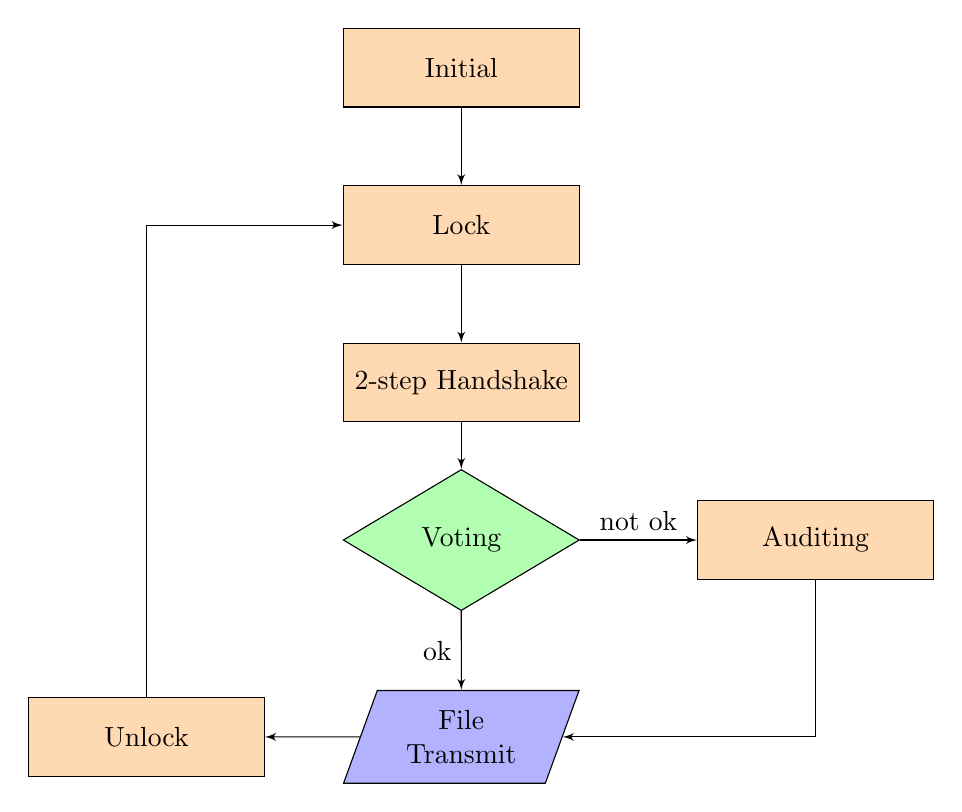
\begin{tikzpicture}[node distance=2cm]
		%定义流程图具体形状
		\node (init) [process] {Initial};
		\node (lock) [process, below of=init] {Lock};
		\node (twostep) [process, below of=lock] {2-step Handshake};
		\node (voting) [decision, below of=twostep] {Voting};
		\node (update) [io, below of=voting, align=center, yshift=-0.5cm] {File \\ Transmit};
		\node (auditing) [process, right of=voting, xshift=2.5cm] {Auditing};
		\node (unlock) [process, left of=update, xshift=-2cm] {Unlock};

		%连接具体形状
		\path [line](init) -- (lock);
		\path [line](lock) -- (twostep);
		\path [line](twostep) -- (voting);
		\path [line](voting) -- node[anchor=east] {ok} (update);
		\path [line](voting) -- node[anchor=south] {not ok} (auditing);
		\path [line](auditing) |- (update);
		\path [line](update) -- (unlock);
		\path [line](unlock) |- (lock);
		\end{tikzpicture}%
	}
	\end{center}
\end{frame}

\subsection{Initial}
\begin{frame}{Initial}
	\alert{File $\rightarrow$ Merkle Tree}\\
	\begin{center}
	\includegraphics[width=1\textwidth]{init.png}
	\end{center}
\end{frame}

\subsection{Read}
\begin{frame}{READ}{\RNum{1}. 2-step Handshake}
	\begin{center}
	\includegraphics[width=.85\textwidth]{Read1.png}
	\end{center}
\end{frame}

\begin{frame}{READ}{\RNum{2}. Voting}
	\begin{center}
	\includegraphics[width=.65\textwidth]{Read2.png}
	\end{center}
\end{frame}

\begin{frame}{READ}{\RNum{3}. Download}
	\begin{center}
	\includegraphics[width=.85\textwidth]{Read3.png}
	\end{center}
\end{frame}

\subsection{Write}
\begin{frame}{WRITE}{\RNum{1}. Upload}
	\begin{center}
	\includegraphics[width=.95\textwidth]{Write1.png}
	\end{center}
\end{frame}

\begin{frame}{WRITE}{\RNum{2}. Update Merkle Tree}
	\begin{center}
	\includegraphics[width=.65\textwidth]{Write2.png}
	\end{center}
\end{frame}

\begin{frame}{WRITE}{\RNum{3}. Voting}
	\begin{center}
	\includegraphics[width=.85\textwidth]{Write3.png}
	\end{center}
\end{frame}

\subsection{Audit}
\begin{frame}{AUDIT}{\RNum{1}. Download and Check LastReq}
	\begin{center}
	\includegraphics[width=.85\textwidth]{Audit1.png}
	\end{center}
\end{frame}

\begin{frame}{AUDIT}{\RNum{2}. Download Roothash or Merkle Tree}
	\begin{center}
	\includegraphics[width=.65\textwidth]{Audit2.png}
	\end{center}
\end{frame}

\begin{frame}[fragile]{AUDIT}{\RNum{3}. Auditing}
	\begin{center}
	\begin{minipage}{.9\hsize}
	\begin{lstlisting}[mathescape, language=Java, caption=Audit algorithm]
	AUDIT(lastAck)
	$\tab{}$op $\leftarrow$ lastAck.req.op
	$\tab{}$if op.type = DOWNLOAD
	$\tab{}$$\tab{}$success $\leftarrow$ roothash.equals(lastAck.result)
	$\tab{}$if op.type = UPLOAD
	$\tab{}$$\tab{}$merkleTreeOld.update(op.msg)
	$\tab{}$$\tab{}$success $\leftarrow$ roothash.equals(lastAck.result)
	$\tab{}$return success
	\end{lstlisting}
	\end{minipage}
	\end{center}
\end{frame}

\section{Implement Steps}
\begin{frame}{Implement Steps}
	\begin{enumerate}
	{\color{blue}
	\item Hash Handle : create, update, delete
	\item Operation Handle : read, write, audit
	\item File Transmit : send, receive
	\item Merkle Tree Transmit : serialize}
	\item \alert{\it Instant Auditing of Cloud Storage Access by Cache Partial Merkle tree}
	\item Run on Real Cloud Environment (VM)
	\end{enumerate}
\end{frame}

\section{Experimental Results}
\begin{frame}{Create Merkle Tree}
	\begin{center}
	\begin{tabu}{cccc}
	\rowfont{\color{blue} \scriptsize} {Account A} & {666 MB}  & {42 files}     & {6 directories}    \\
	\rowfont{\color{blue} \scriptsize} {Account B} & {34 MB}   & {54192 files}  & {188 directories}  \\
	\rowfont{\color{blue} \scriptsize} {Account C} & {6.54 GB} & {58484 files}  & {1718 directories} \\
	\rowfont{\color{blue} \scriptsize} {Account D} & {20.6 GB} & {175389 files} & {5154 directories} \\
	\end{tabu}
	\end{center}
	\begin{table}[]
	\centering
	\captionsetup{justification=centering}
	\caption{\tiny TIMES REQUIRED TO GENERATE THE ROOT HASH FROM NOT-HASHED FILES (IN SECONDS)}
	\begin{tabular}{|c|c|c|c|}
	\hline
	{\bf Account} & {\bf Senior}  & {\bf My}      & {\bf MerkleTree Size} \\ \hline
	{\bf A}       & {\it 3.404}   & {\it 3.645}   & {3.74 KB}             \\ \hline
	{\bf B}       & {\it 16.618}  & {\it 7.669}   & {3.77 MB}             \\ \hline
	{\bf C}       & {\it 229.351} & {\it 242.198} & {4.30 MB}             \\ \hline
	{\bf D}       & {\it }        & {\it 815.408} & {12.9 MB}             \\ \hline
	\end{tabular}\\
	\end{table}
\end{frame}
\begin{frame}{Operation Processing Time}
	\begin{table}[]
	\makebox[0pt][c]{\parbox{\textwidth}{%
	\begin{minipage}{.47\hsize}
	\captionsetup{justification=centering}
	\caption{DOWNLOAD TIME (ms)}
	\begin{tabu}{|c|c|c|}
	\hline
	\rowfont{\color{blue}} {\bf Account} & {\bf 100 times} & {\bf Audit$^*$} \\ \hline
	\rowfont{\color{blue}} {\bf A}       & {\it 4635}      & {\it 34 + 0}    \\ \hline
	\rowfont{\color{blue}} {\bf B}       & {\it 4660}      & {\it 33 + 0}    \\ \hline
	\rowfont{\color{blue}} {\bf C}       & {\it 5429}      & {\it 31 + 0}    \\ \hline
	\rowfont{\color{blue}} {\bf D}       & {\it 5554}      & {\it 31 + 0}    \\ \hline
	\end{tabu}
	\end{minipage}
	\begin{minipage}{.53\hsize}
	\captionsetup{justification=centering}
	\caption{UPLOAD TIME (ms)}
	\begin{tabular}{|c|c|c|}
	\hline
	{\bf Account} & {\bf 100 times} & {\bf Audit$^*$}   \\ \hline
	{\bf A}       & {\it 4322}      & {\it 41  + 7}     \\ \hline
	{\bf B}       & {\it 5643}      & {\it 421 + 997}   \\ \hline
	{\bf C}       & {\it 9236}      & {\it 421 + 2621}  \\ \hline
	{\bf D}       & {\it 11466}     & {\it 1263 + 8085} \\ \hline
	\end{tabular}
	\end{minipage}
	}}
	\footnote{* download attestations time + audit time}
	\end{table}	
\end{frame}
\end{CJK}
\end{document}
